\section{Data}\label{Sec:Data}

For the analysis explained in this paper data was downloaded for a website independent from airbnb itself. insideairbnb (\href{http://insideairbnb.com/}{insideairbnb.com}) scrapes (????) airbnb to get its data and posts it online for the public to use on own analysis, while also providing some analysis of its own.
\\
The data is divided according to cities and for each there is general information about the city's properties and their availability for the next year. The variables that are being kept for this analysis are listing on table 1. (HOW TO MAKE IT CHANGE NUMBER???).

\iffalse

\begin{table}[H]
\centering
\begin{tabular}{l}
  \hline
x \\ 
  \hline
id \\ 
  attraction\_count \\ 
  attraction\_dist \\ 
  station\_count \\ 
  station\_dist \\ 
  long \\ 
  lat \\ 
  price \\ 
  property\_type \\ 
  room\_type \\ 
  security\_deposit\_yn \\ 
  cleaning\_fee\_yn \\ 
  host\_is\_superhost \\ 
  accommodates \\ 
  bedrooms \\ 
  beds \\ 
  minimum\_nights \\ 
  review\_scores\_rating \\ 
  number\_of\_reviews \\ 
  reviewed\_yn \\ 
  cancellation\_policy \\ 
  availability\_30 \\ 
  availability\_60 \\ 
  availability\_90 \\ 
  availability\_365 \\ 
  listing\_url \\ 
  district \\ 
  vbb\_area \\ 
  neighbourhood \\ 
  2018\_fall\_availability \\ 
  2018\_winter\_availability \\ 
  2019\_spring\_availability \\ 
  2019\_summer\_availability \\ 
  2019\_fall\_availability \\ 
  2019\_winter\_availability \\ 
   \hline
\end{tabular}
\end{table}

\fi

\subsection{Berlin neighbourhoods and districts}


Berlin consists of 96 neighbourhoods (Ortsteile), which are grouped into 12 districts (Bezirke).

\begin{table}[H]
\centering
\begin{tabular}{ll}
  \hline \hline
Neighbourhood & District \\ 
  \hline
Charlottenburg & Charlottenburg-Wilmersdorf \\ 
  Wilmersdorf & Charlottenburg-Wilmersdorf \\ 
  Grunewald & Charlottenburg-Wilmersdorf \\ 
  Westend & Charlottenburg-Wilmersdorf \\ 
  Schmargendorf & Charlottenburg-Wilmersdorf \\ 
  Charlottenburg-Nord & Charlottenburg-Wilmersdorf \\ 
  Halensee & Charlottenburg-Wilmersdorf \\ 
  Friedrichshain & Friedrichshain-Kreuzberg \\ 
  Kreuzberg & Friedrichshain-Kreuzberg \\ 
  Friedrichsfelde & Lichtenberg \\ 
  Karlshorst & Lichtenberg \\ 
  Malchow & Lichtenberg \\ 
  Wartenberg & Lichtenberg \\ 
  Falkenberg & Lichtenberg \\ 
  Fennpfuhl & Lichtenberg \\ 
  Lichtenberg & Lichtenberg \\ 
  Neu-Hohenschönhausen & Lichtenberg \\ 
  Alt-Hohenschönhausen & Lichtenberg \\ 
  Rummelsburg & Lichtenberg \\ 
  Marzahn & Marzahn-Hellersdorf \\ 
  Biesdorf & Marzahn-Hellersdorf \\ 
  Kaulsdorf & Marzahn-Hellersdorf \\ 
  Mahlsdorf & Marzahn-Hellersdorf \\ 
  Hellersdorf & Marzahn-Hellersdorf \\ 
  Mitte & Mitte \\ 
  Moabit & Mitte \\ 
  Hansaviertel & Mitte \\ 
  Gesundbrunnen & Mitte \\ 
  Tiergarten & Mitte \\ 
  Wedding & Mitte \\ 
  Buckow & Neukölln \\ 
  Buckow & Neukölln \\ 
  Gropiusstadt & Neukölln \\ 
  Neukölln & Neukölln \\ 
  Britz & Neukölln \\ 
  Rudow & Neukölln \\ 
  Blankenfelde & Pankow \\ 
  Buch & Pankow \\ 
  Wilhelmsruh & Pankow \\ 
  Prenzlauer Berg & Pankow \\ 
  Weißensee & Pankow \\ 
  Blankenburg & Pankow \\ 
  Heinersdorf & Pankow \\ 
  Karow & Pankow \\ 
  Stadtrandsiedlung Malchow & Pankow \\ 
  Pankow & Pankow \\ 
  Französisch Buchholz & Pankow \\ 
  Niederschönhausen & Pankow \\ 
  Rosenthal & Pankow \\ 
  Konradshöhe & Reinickendorf \\ 
  Tegel & Reinickendorf \\ 
  Märkisches Viertel & Reinickendorf \\ 
  Hermsdorf & Reinickendorf \\ 
  Borsigwalde & Reinickendorf \\ 
  Lübars & Reinickendorf \\ 
  Reinickendorf & Reinickendorf \\ 
  Heiligensee & Reinickendorf \\ 
  Frohnau & Reinickendorf \\ 
  Waidmannslust & Reinickendorf \\ 
  Wittenau & Reinickendorf \\ 
  Gatow & Spandau \\ 
  Kladow & Spandau \\ 
  Falkenhagener Feld & Spandau \\ 
  Wilhelmstadt & Spandau \\ 
  Spandau & Spandau \\ 
  Haselhorst & Spandau \\ 
  Siemensstadt & Spandau \\ 
  Staaken & Spandau \\ 
  Hakenfelde & Spandau \\ 
  Steglitz & Steglitz-Zehlendorf \\ 
  Lichterfelde & Steglitz-Zehlendorf \\ 
  Lankwitz & Steglitz-Zehlendorf \\ 
  Zehlendorf & Steglitz-Zehlendorf \\ 
  Dahlem & Steglitz-Zehlendorf \\ 
  Nikolassee & Steglitz-Zehlendorf \\ 
  Wannsee & Steglitz-Zehlendorf \\ 
  Friedenau & Tempelhof-Schöneberg \\ 
  Schöneberg & Tempelhof-Schöneberg \\ 
  Tempelhof & Tempelhof-Schöneberg \\ 
  Mariendorf & Tempelhof-Schöneberg \\ 
  Marienfelde & Tempelhof-Schöneberg \\ 
  Lichtenrade & Tempelhof-Schöneberg \\ 
  Alt-Treptow & Treptow-Köpenick \\ 
  Plänterwald & Treptow-Köpenick \\ 
  Johannisthal & Treptow-Köpenick \\ 
  Adlershof & Treptow-Köpenick \\ 
  Köpenick & Treptow-Köpenick \\ 
  Rahnsdorf & Treptow-Köpenick \\ 
  Müggelheim & Treptow-Köpenick \\ 
  Schmöckwitz & Treptow-Köpenick \\ 
  Bohnsdorf & Treptow-Köpenick \\ 
  Baumschulenweg & Treptow-Köpenick \\ 
  Niederschöneweide & Treptow-Köpenick \\ 
  Altglienicke & Treptow-Köpenick \\ 
  Oberschöneweide & Treptow-Köpenick \\ 
  Friedrichshagen & Treptow-Köpenick \\ 
  Grünau & Treptow-Köpenick \\ 
   \hline \hline
\end{tabular}
\caption{Berlin's Neighbourhoods and Districts}
\end{table}

The polygons to plot them are extracted from the relative shapefile which is loaded with the function st\_read from the \texttt{sf} package to have it already as a sf polygon. 

\lstinputlisting[language=R, firstline=13, lastline=14, firstnumber=1, escapechar=|, caption={|\textbf{\href{https://github.com/silvia-ventoruzzo/SPL-WISE-2018/blob/master/Berlin_Districts_Neighbourhoods/berlin_districts_neighbourhoods.R}{berlin\_districts\_neighbourhoods.R}}|}]{../Berlin_Districts_Neighbourhoods/berlin_districts_neighbourhoods.R}

The types of objects used by and created with this package come in very handy since they look like data frames and many functions for data frames can be used on them. 

\begin{table}[H]
\centering
\begin{tabular}{lll}
  \hline \hline
                  Name &                       BEZNAME &          geometry \\ 
  \hline
Buckow              : 2   & Treptow-Köpenick          :15   & POLYGON      :97   \\ 
  Adlershof           : 1   & Pankow                    :13   & epsg:4326    : 0   \\ 
  Alt-Hohenschönhausen: 1   & Reinickendorf             :11   & +proj=long...: 0   \\ 
  Alt-Treptow         : 1   & Lichtenberg               :10   &  \\ 
  Altglienicke        : 1   & Spandau                   : 9   &  \\ 
  Baumschulenweg      : 1   & Charlottenburg-Wilmersdorf: 7   &  \\ 
  (Other)             :90   & (Other)                   :32   &  \\ 
   \hline \hline
\end{tabular}
\end{table}

Since the polygons represent the neighbourhoods, we do not need to perform any transformation on this object. Here we keep only the variables of interest, rename them and reorder the rows.

\lstinputlisting[language=R, firstline=16, lastline=26, firstnumber=4, escapechar=|, caption={|\textbf{\href{https://github.com/silvia-ventoruzzo/SPL-WISE-2018/blob/master/Berlin_Districts_Neighbourhoods/berlin_districts_neighbourhoods.R}{berlin\_districts\_neighbourhoods.R}}|}]{../Berlin_Districts_Neighbourhoods/berlin_districts_neighbourhoods.R}

However, we have the problem with the neighbourhood Buckow, is composed of two separate
parts. Therefore we need to unite the neighbourhoods according to their name. In this way we obtain an sf object with 96 polygons, the one of Buckow being a list of polygons.

\lstinputlisting[language=R, firstline=28, lastline=32, firstnumber=15, escapechar=|, caption={|\textbf{\href{https://github.com/silvia-ventoruzzo/SPL-WISE-2018/blob/master/Berlin_Districts_Neighbourhoods/berlin_districts_neighbourhoods.R}{berlin\_districts\_neighbourhoods.R}}|}]{../Berlin_Districts_Neighbourhoods/berlin_districts_neighbourhoods.R}

For the districts we perform the same procedure, but this time we unite the polygons only by their district, which are represented here by the group variable.

\subsection{Berlin VBB Areas}

The VBB (Verkehrsverbund Berlin-Brandenburg) is "the public transport authority covering the federal states of Berlin and Brandenburg" (CITATION: \href{https://www.vbb.de/en/about-us/the-company-vbb}{VBB Website}). The city of Berlin, in particular, is divided in two fare areas: A, covering the center of Berlin up to the Ringbahn (circular line), and B, from the Ringbahn to the border with Brandenburg. After that there is also the area C, which however will not be covered here since we only consider the city of Berlin.

\begin{figure}[H]
\begin{center}
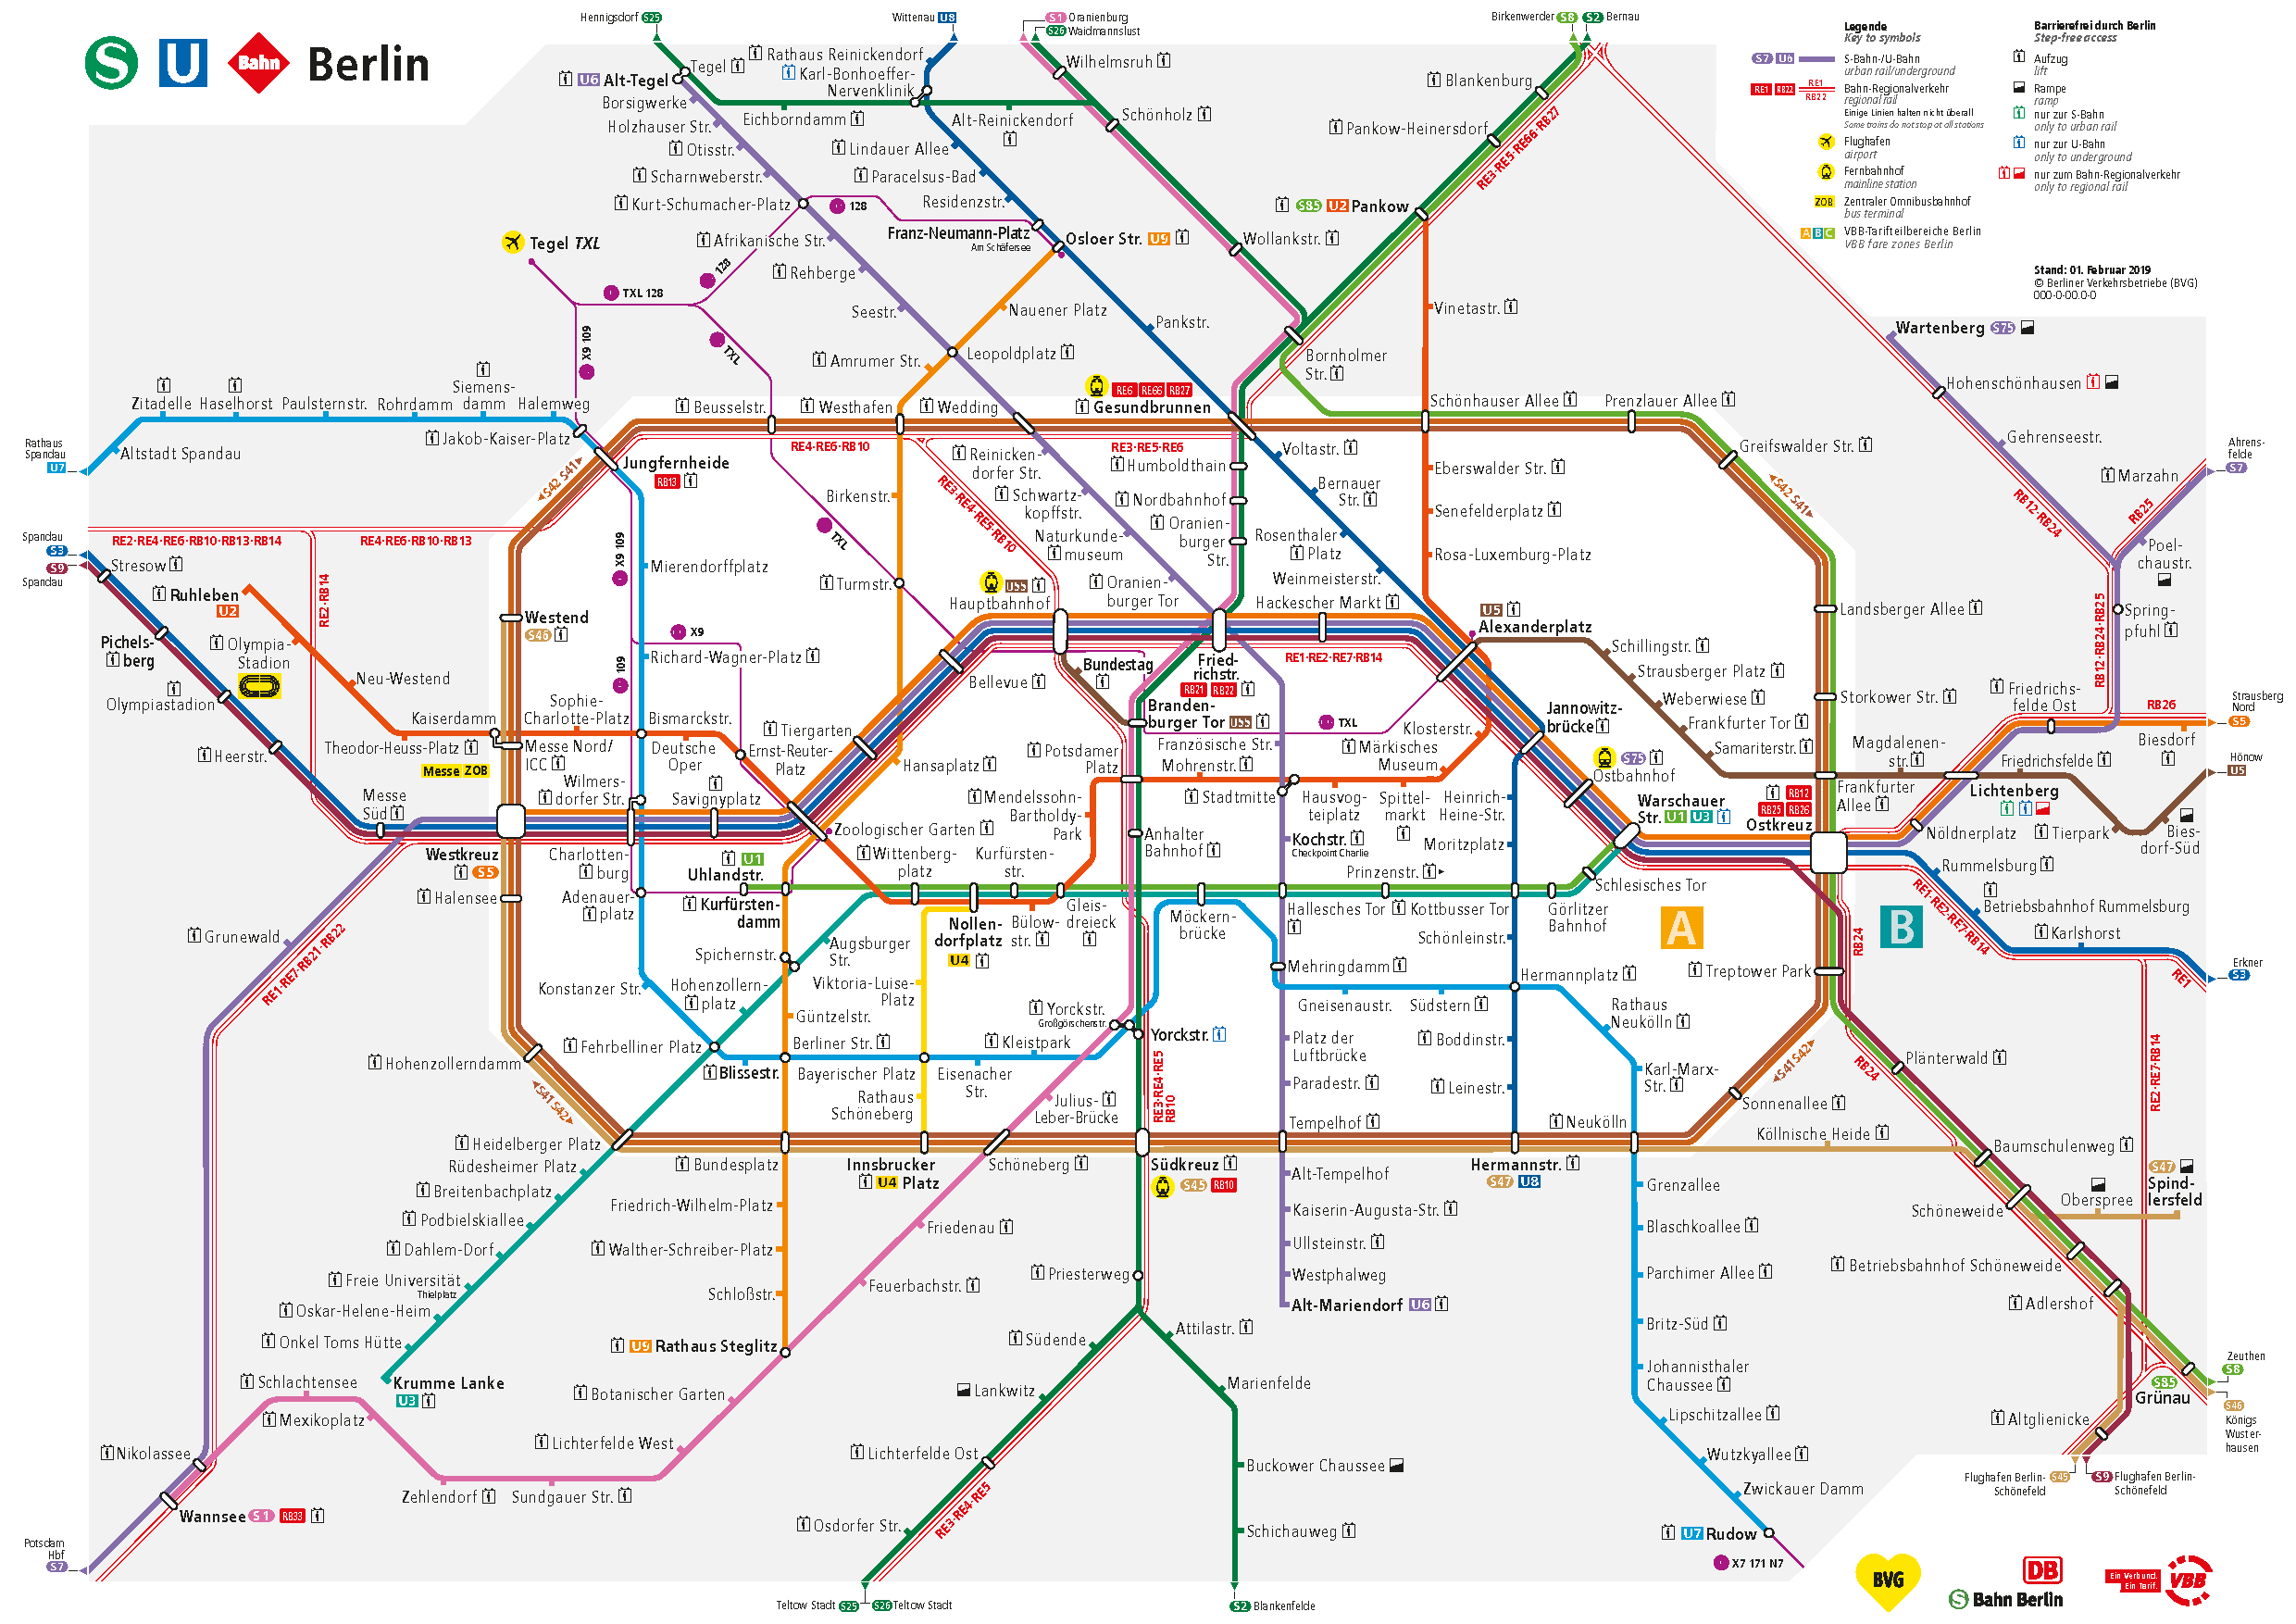
\includegraphics[width=0.8\textwidth, keepaspectratio]{S_und_U-Bahnnetz_mit_Regionalbahn_Innenstadt.pdf} \\
\caption{Network Map of Berlin Areas A and B (from \href{https://www.vbb.de/en/timetables/network-maps}{VBB Website})}
\end{center}
\end{figure}

We tried to replicate these areas by using the Berlin polygons and the stations points.

\lstinputlisting[language=R, firstline=16, lastline=18, firstnumber=1, escapechar=|, caption={|\textbf{\href{https://github.com/silvia-ventoruzzo/SPL-WISE-2018/blob/master/Berlin_Districts_Neighbourhoods/berlin_districts_neighbourhoods.R}{berlin\_vbb\_areas.R}}|}]{../Berlin_VBB_Areas/berlin_vbb_areas.R}